%!TEX root =  main.tex
\section{The centralized partitioning scheme}

\fp{Here we should describe the new scheme, which computes partitions on the fly based on feedback from the oracle}

\eb{Hint at the possible benefits of using graph partitioning to distribute objects across partitions (i.e., make the link to the next subsection).}

%EF: Link with GP
If the system can be modelled as a graph, as described in the previous session, we can take advantage of algorithms that perform graph partitioning to optimise the state partitioning of \ssmr\  while using concepts from \dssmr. The problem of graph partitioning is well stablished and despite being NP-Complete \ref{NPC_GraphPartition}, several approximation algorithms exist. First we define what graph partitioning is and how it can analysed to our needs, next we explore possibilities that are easily obtainable when applying the same graph's reasoning.

\subsection{Graph partitioning}
%EF: What is graph partitioning?
Graph partitioning is an important subproblem of any system that aims parallelization and thus scalability, a bad partitioning can undermine all effort done in other parts of the system, so having the data well and evenly distributed is fundamental.


%EF:  Need to relate the objects to the graph so it makes sense to use already functioning graph partitioning algorithms.

%EF:  Definition of Graph partitioning
Given a graph $G = (V, E)$, and a number of partitions $k$, a partition $p_i$ with $1 \leq i \leq k$ is a subset of $V$ such that $\bigcup p_i = V$ and $\bigcap p_i = \emptyset$. That's it, the graph is partitioned in $k$ servers, each one with its respective replicas, all the objects are maintained partitioned among the replica.

%EF:  What is a good partitioning? Our definition:
We define a good partitioning as one that minimize the cross-edges among partitions while maintaining each partition balanced, more formally, let $C(P)$ be a set of edges connecting a vertex in $P$ with a vertex in $V - P$, ideally $\frac{\sum_{i=1}^{k}|C(p_i)|}{|E|} = 0$ and $\frac{max_{1 \leq i \leq k}(|p_i|)}{avg_{1 \leq i \leq k}(|p_i|)} = 1$





%EF: Partitioning 
In \appname, the partitioning 

\subsection{Dynamic repartitioning}
%EF:  Why do we want that?
The ability to execute a repartition on-the-fly is crucial to systems that 

\begin{figure}
	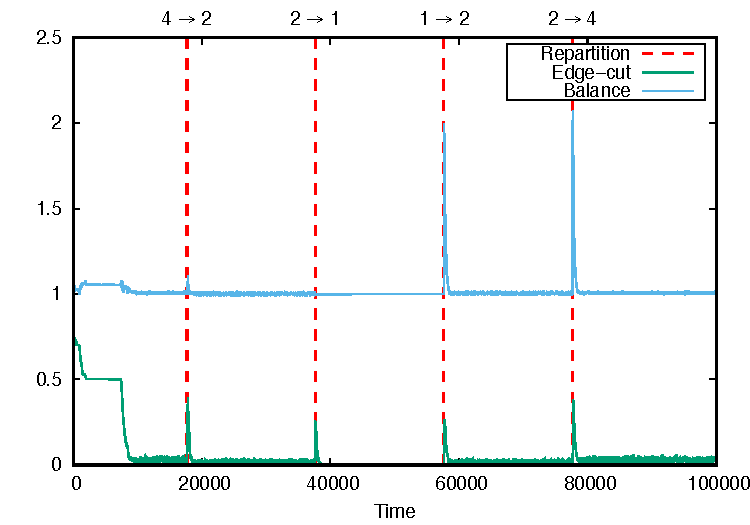
\includegraphics[width=1.0\linewidth]{graphs/0.01_edgecuts/repartition/4-2-1-2-4/edge_cut_balance_max_4_part}
	\caption{Multiple repartitioning in the same execution.}
	\label{fig:repartition_4_times}
\end{figure}

%EF:  How do we do a repartitioning?
Whenever an external agent or the oracle itself decide that there should be a new partitioning, a \emph{Partition} command is sent to the oracle, which executes the respective step in algorithm~\ref{alg:oracle_partition}. The system continues to operate normally while the partitioning is taking place.

%EF: What if a client is caught in the middle of repartitioning
When a client issues a command and a repartitioning was applied before, like seen in figure~\ref{fig:oracle_repartition}, that command will fail and the client is going to be requested to update the version of its cache to the one replied by the oracle.


\begin{algorithm}[t!]
    \small

    \begin{distribalgo}[1]

        \vspace{1.5mm}

        \INDENT{\emph{Initialization:}}
            \STATE $round: 0$
            \STATE $new\_partitioning_{r}: \emptyset$
            \STATE $rcvd\_applies_{r} \leftarrow \emptyset$

        \ENDINDENT
        \vspace{1.5mm}
        \INDENT{Each oracle partition $o \in \oom$ does:}
            \vspace{1.5mm}
            \INDENT{\textbf{when} $receive(Partition)$}
                \STATE $round \leftarrow round + 1$
                \STATE $new\_partitioning_{round} \leftarrow$ partitioner($o.graph$)
                \STATE \rmcast$(\oom, Apply(round))$
            \ENDINDENT

            \vspace{1.5mm}

            \INDENT{\textbf{when} \rmdel$(Apply(round))$ from partition $o'$}
                \STATE $rcvd\_applies_{round} \leftarrow rcvd\_applies_{round} \cup o'$
                \IF{$rcvd\_applies_{round} \cap \oom = \emptyset$}
                    \STATE \amcast$(\oom, Apply(round))$
                \ENDIF
            \ENDINDENT

            \vspace{1.5mm}
            
             \INDENT{\textbf{when} \amdel$(Apply(round))$}
                \STATE $o.partitioning \leftarrow new\_partitioning_{round}$
            \ENDINDENT

        \ENDINDENT

    \vspace{1.7mm}

    \textbf{Algorithm variables:}

    \vspace{1.25mm}

    partitioner: An external partition algorithm

    \vspace{1.25mm}

    \oo: The set of oracle partitions

    \vspace{1mm}

    $o.graph$: The graph stored in the oracle

    \vspace{1mm}

    $o.partitioning$: The current graph partitioning

    \caption{Oracle's partitioning}
    \label{alg:oracle_partition}
\end{distribalgo}
\end{algorithm}


\begin{figure*}
\begin{minipage}[b]{1\linewidth} % A minipage that covers the whole width of the page
\centering
      \includegraphics[width=1.0\linewidth]{figures/repartitioning}
\end{minipage}
\caption{How commands are treated in case of a repartitioning in the oracle.}
\label{fig:oracle_repartition}
\end{figure*}
